\section{Результаты измерений}
\begin{table}[!ht]
    \centering
    \begin{tabular}{|l|l|l|}
    \hline
        $\tau$ & $\Delta h_1$ & $\Delta h_2$ \\ \hline
        5 & 10.4 & 1.5 \\ \hline
        10 & 10.7 & 1.2 \\ \hline
        15 & 10.8 & 1.1 \\ \hline
        20 & 10.9 & 0.9 \\ \hline
        25 & 10.8 & 0.8 \\ \hline
        30 & 10.8 & 0.7 \\ \hline
        35 & 10.7 & 0.5 \\ \hline
    \end{tabular}
\end{table}

\begin{figure}[ht!]
    \centering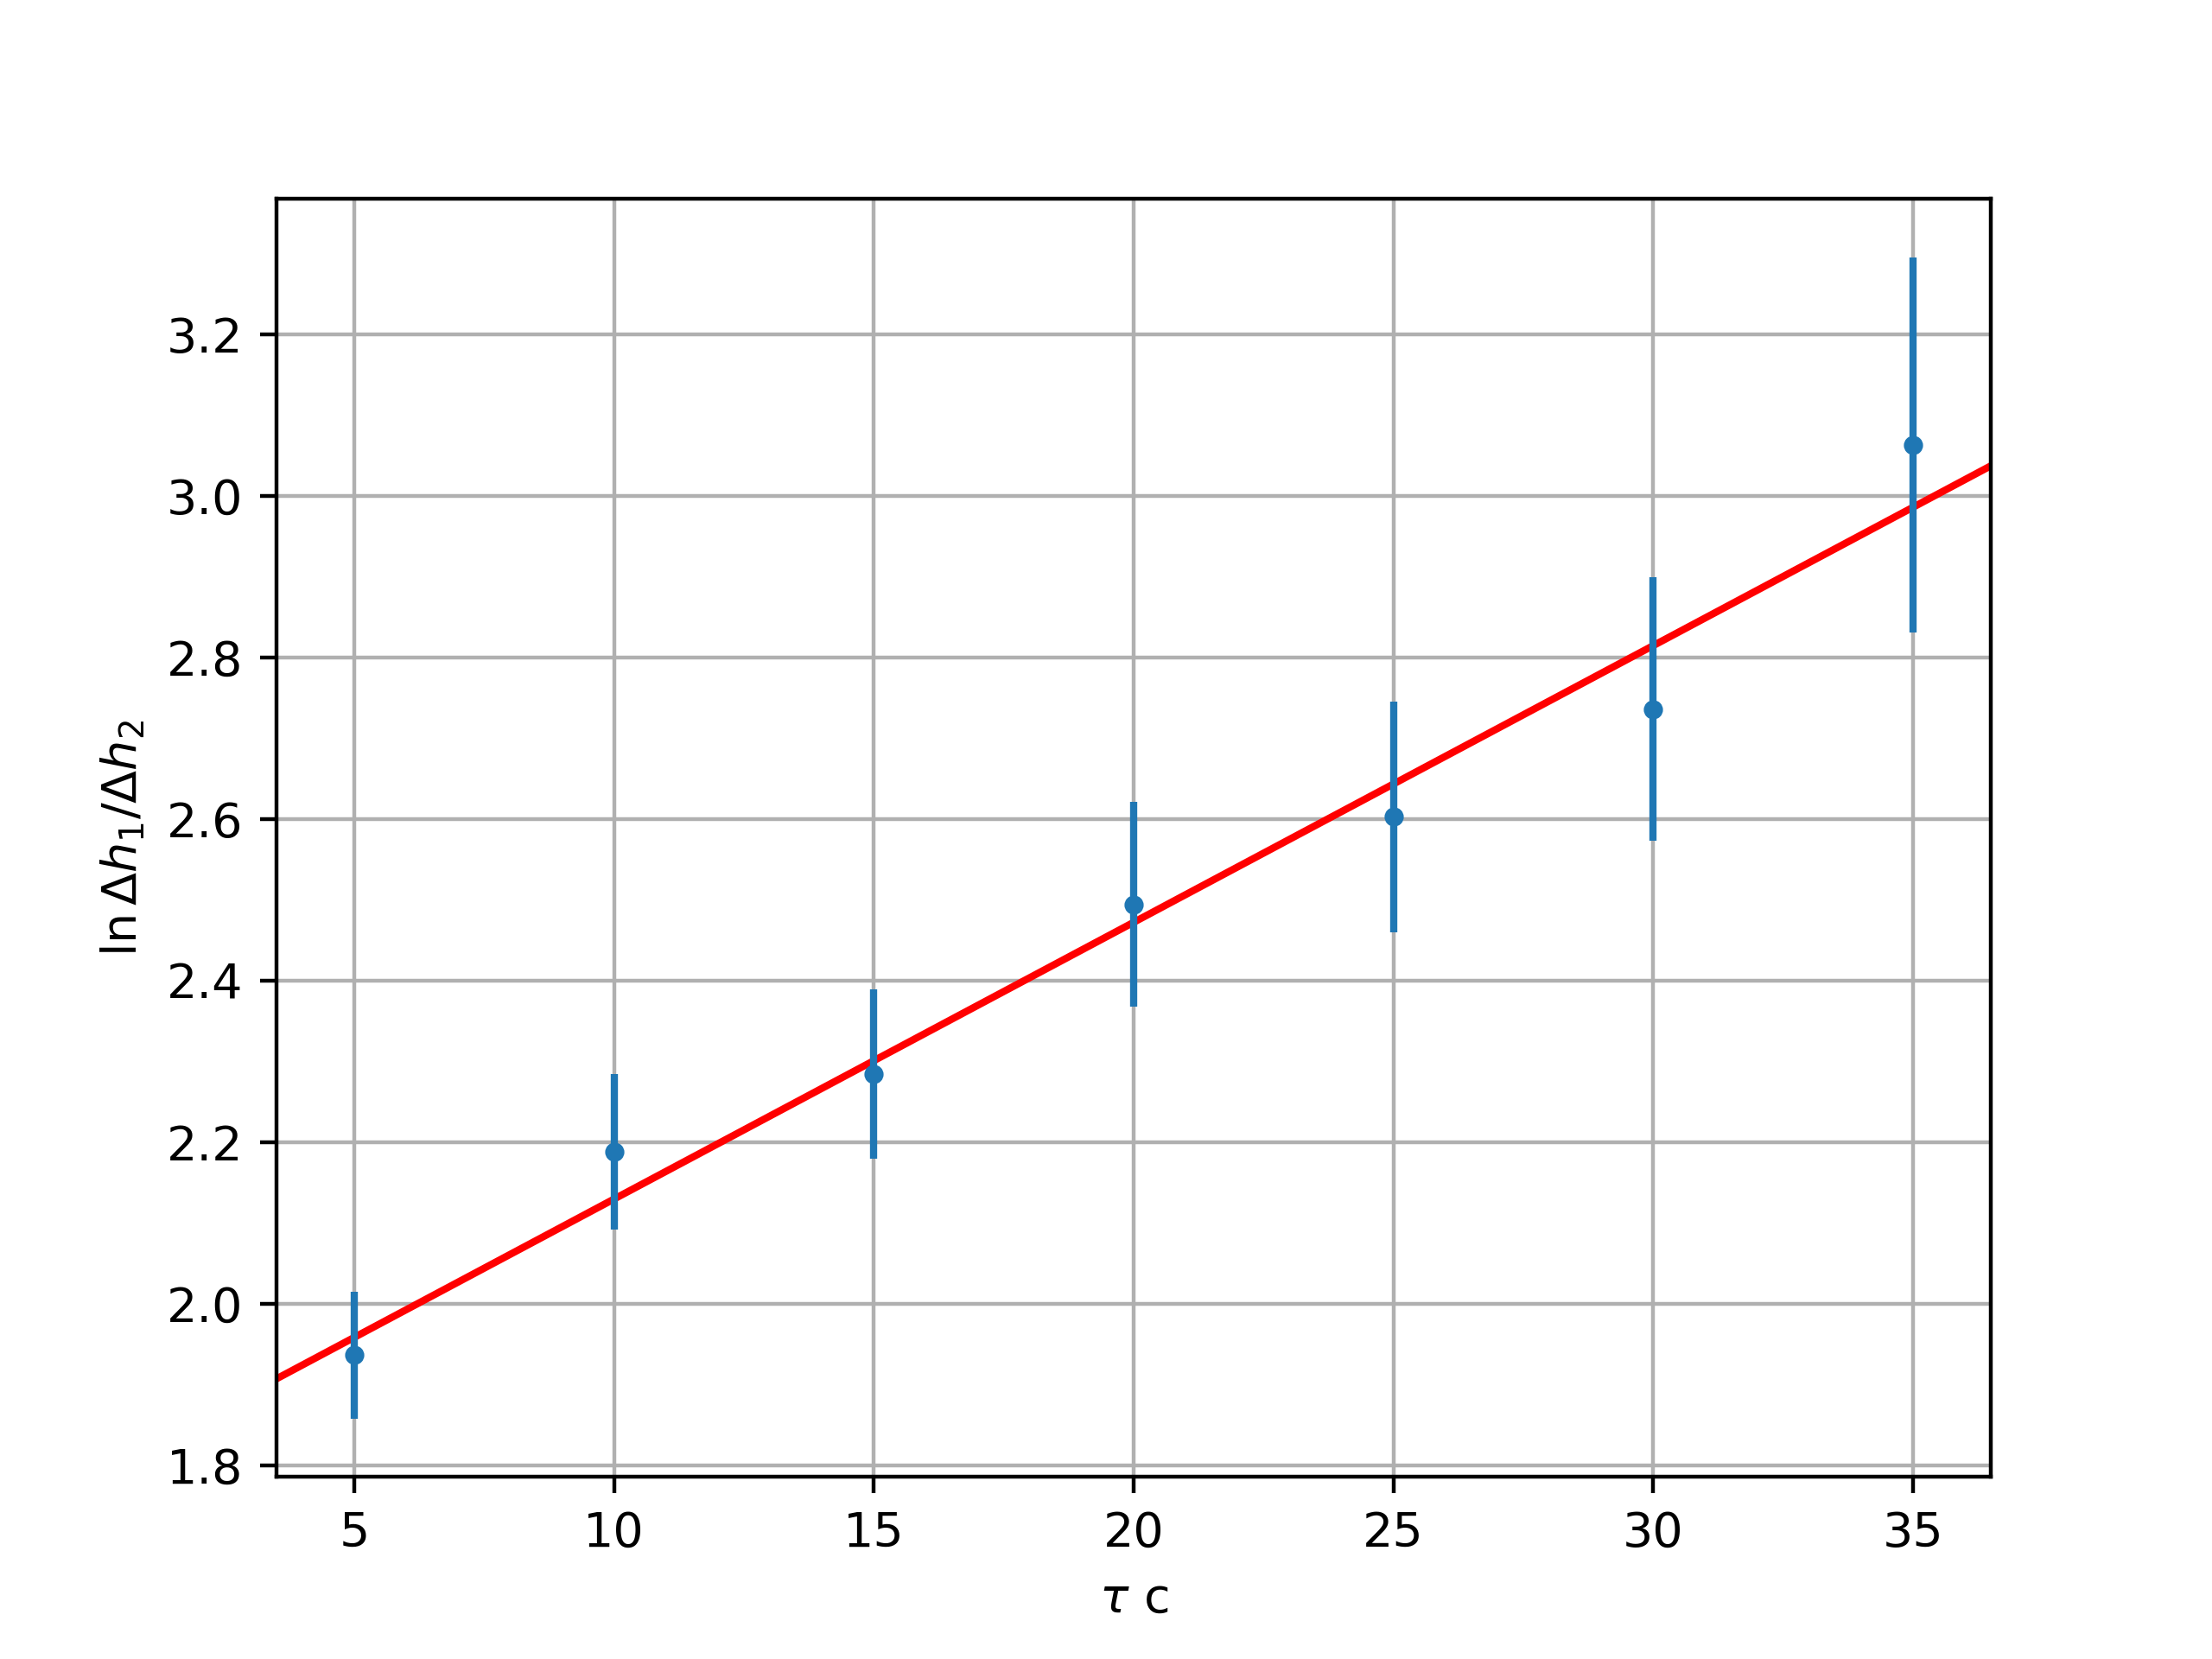
\includegraphics[width=0.8\linewidth]{img/plot.png}
\end{figure}

\[b=1{,}79\pm 0{,}05\,\text{с}^{-1}\]

\[\gamma = \frac{\exp b}{\exp b - 1} = 1{,}2 \pm 0{,}3\]

Табличное значение $\gamma = 9/7 \approx 1{,}3$ лежит в пределах погрешности.

\newpage
